\pagenumbering{Roman}
\setcounter{page}{1}
\lhead{Appendix \thesection}

\begin{appendix}
\section*{Appendix}
\phantomsection
\addcontentsline{toc}{section}{Appendix}
\addtocontents{toc}{\vspace{-0.5em}}

\section{IJulia}
\vspace{1em}
\begin{minipage}{\linewidth}
    \centering
    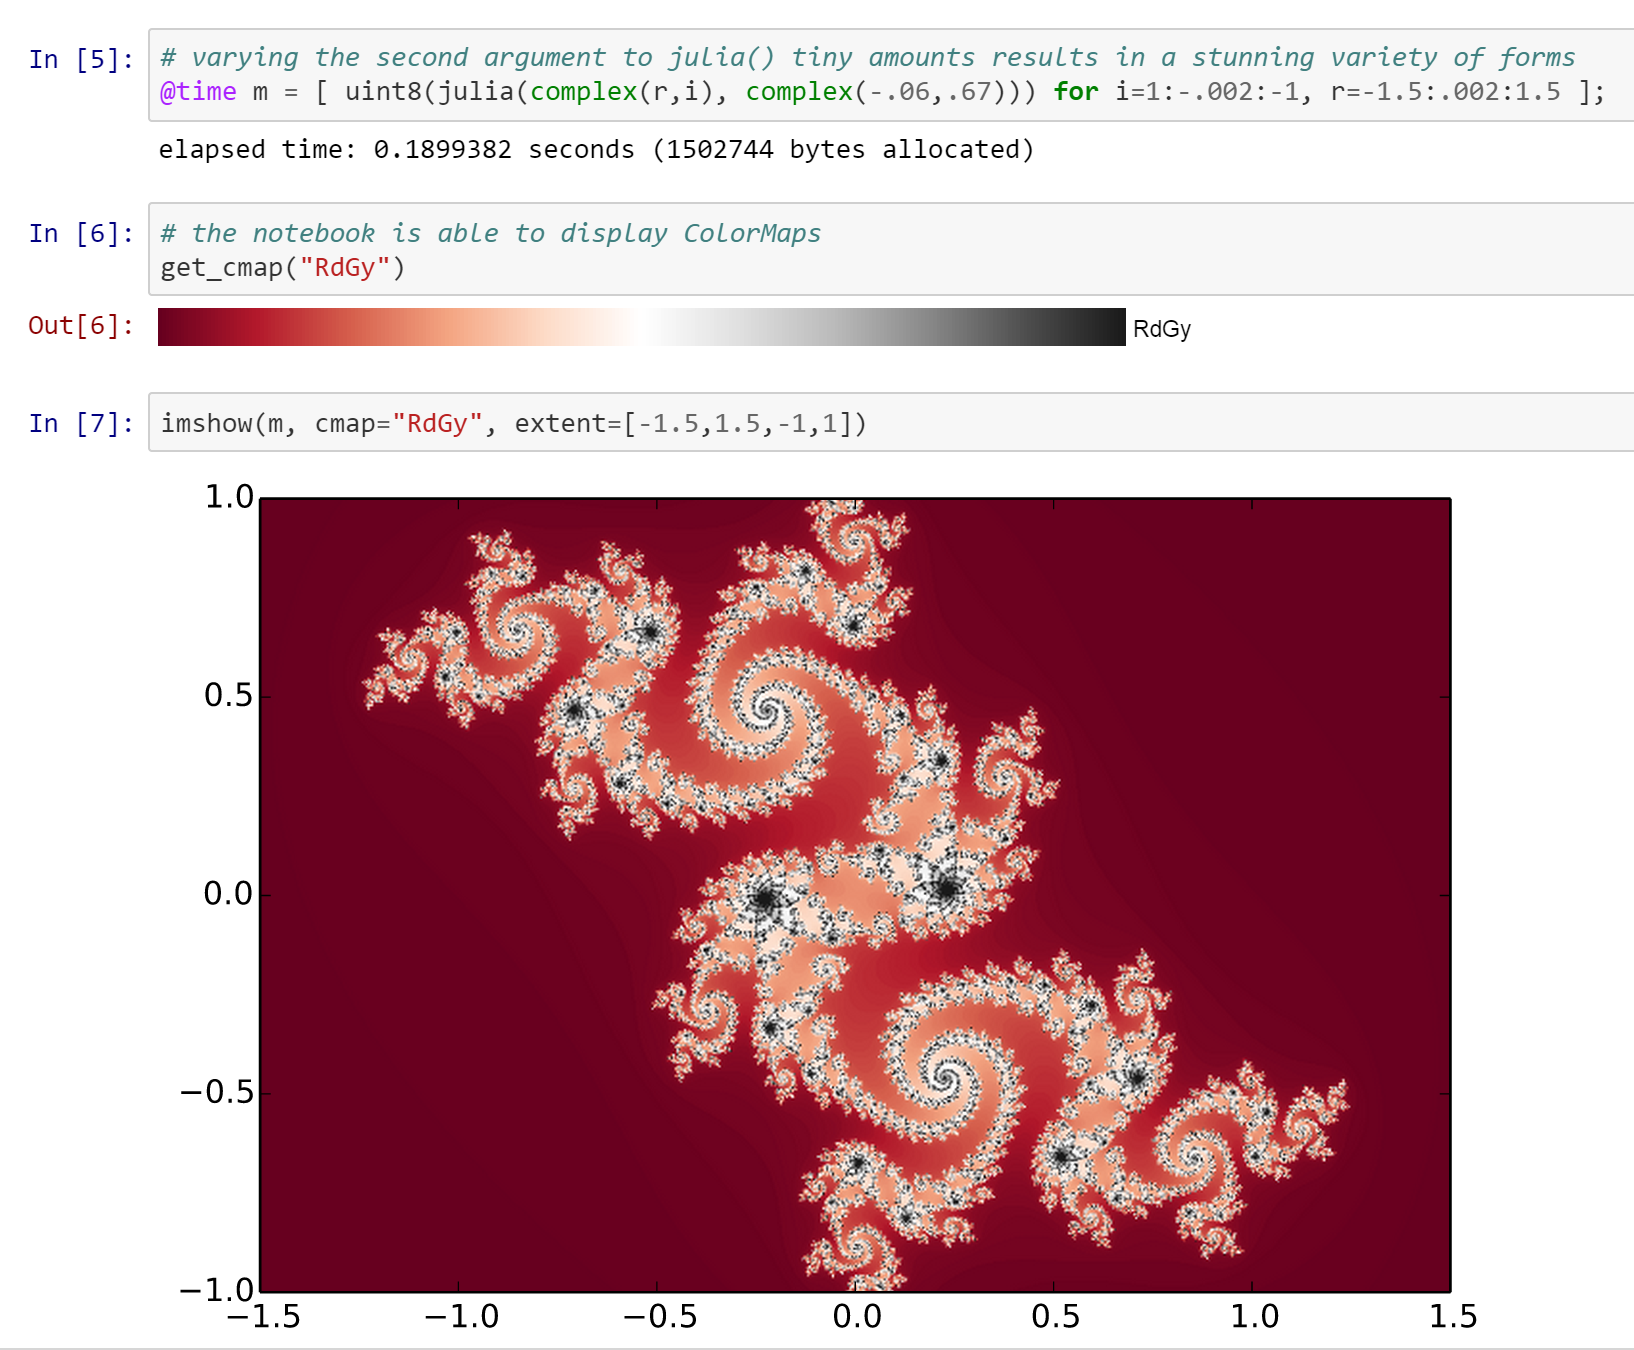
\includegraphics[width=0.9\linewidth]{graphics/ijnotebook.png}
    \captionof{figure}[IJulia Notebook Example]{
        Example of an IJulia Notebooks.
        Screenshot taken from \cite{IJuliaNotebook}
    }
    \label{fig:ijulianotebook}
\end{minipage}

\vspace{1em}
\begin{minipage}{\linewidth}
    \centering
    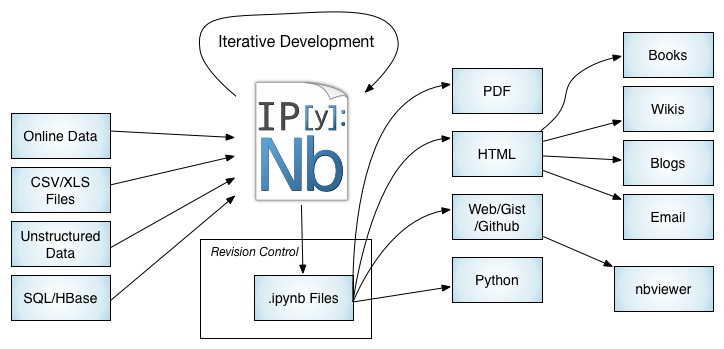
\includegraphics[width=0.9\linewidth]{graphics/IPython_Notebook_Workflows.png}
    \captionof{figure}[IPython Notebook Workflow]{
        Workflow of IPython Notebooks.
        Graphic from Wikipedia \cite{IPyhonNotebookFlow}
    }
    \label{fig:ipythonnotebookflow}
\end{minipage}



\section{GUI}
A nice Appendix.

\subsection*{Screenshot}
\begin{minipage}{\linewidth}
    \centering
    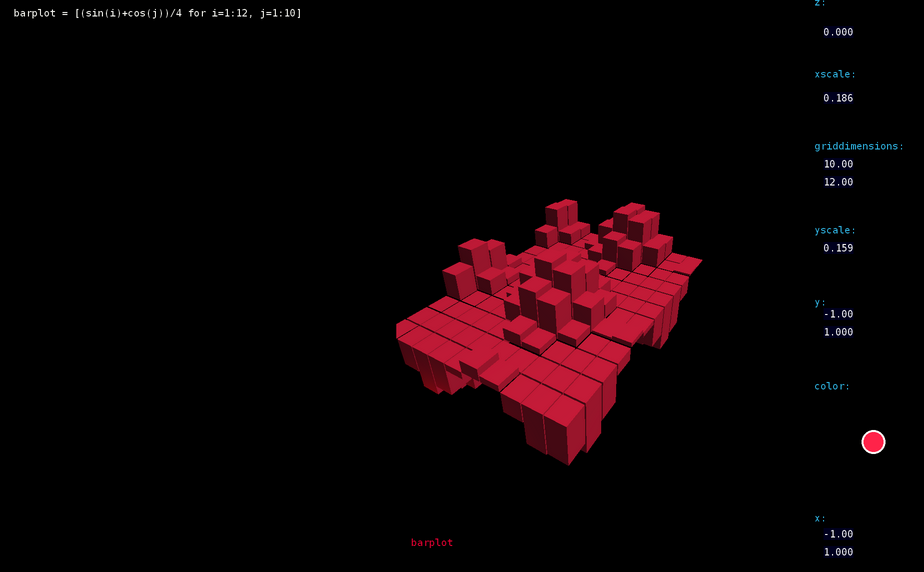
\includegraphics[scale=2.0]{graphics/screenshot.png}
    \captionof{figure}[Prototype]{Screenshot of the prototype. Left: evaluated script, middle: visualization of the variable barplot, right: GUI for editing the parameters of the visualization}
    \label{app:screenshot}
\end{minipage}


\section{Benchmark}

\begin{table}[htb]
\centering
\caption{FE Implementation comparison}
    \sffamily 
    \begin{tabularx}{1.0\textwidth}{l | c | p{5cm}}
        \hline
        implementations         & Language  & Speed in Seconds \\
        \hline
        JFinEALE                & Julia     & 9.6   \\
        Comsol 4.4 with PARDISO & Java      & 16    \\
        Comsol 4.4 with MUMPS   & Java      & 22    \\ 
        Comsol 4.4 with SPOOLES & Java      & 37    \\ 
        FinEALE                 & Matlab    & 810   \\
        \hline
    \end{tabularx} 
    \normalfont
    \label{table:FEComparison}
\end{table}


\end{appendix}
